\section{Experimental Results}
The different approaches used for the classification purpose and the corresponding results are described in the following sections. 
\subsection{Approaches and Settings}

\subsubsection*{k-Nearest Neighbors}
The first classifier we chose is the k-Nearest Neighbors classifier. The
parameter k was obtained by performing a parameter search on a
leave-one-out cross validation. In terms of accuracy, \(k=30\) was
the best choice. The distance measure is euclidean distance, the best
results were obtained without distance weighting.

\subsubsection*{Na\"ive Bayes}
Another approach is the Na\"ive Bayes classifier. Despite some
attributes obviously not being independent, it was still employed
because it proved to be useful in other areas as well.

\subsubsection*{Decision Tree}
We generated a pruned J48-decision tree. The best results were
achieved by using a confidence factor of \(c=0.045\) for pruning the
tree. This value was found by utilizing WEKAs capabilities of linear
parameter search.

\subsubsection*{Neural Network}
A multilayer perceptron is used as a neural network. The structure
consists of 13 input neurons (one for each feature), a hidden layer
of 17 neurons precedes the output layer containing three neurons
(one for each class). A learning rate of \(\alpha=0.1\) is used, a momentum of
\(m=0.1\) is applied in each training step. The number of hidden
neurons was found by conducting a linear search once again, testing
all possible values between zero and 30.

\subsubsection*{Ensemble}
In hope for enhanced results by combining the strenghts of the
different classifiers, all models are combined into an ensemble. The
vote of the whole ensemble is found by conducting a majority voting.

\subsection{Results}
Each classifier as well as the ensemble was evaluated by using 10-fold
cross validation.
As a result, a comparison of the different evaluation metrics can
be found in \fref{fig:result}.

\begin{figure}[h]
	\centering
	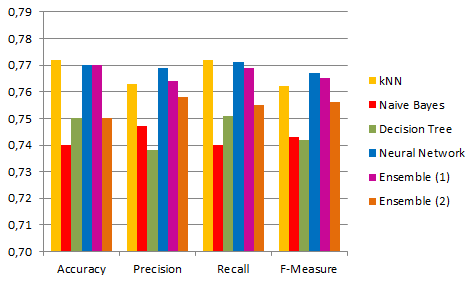
\includegraphics[width=\columnwidth]{../../charts/results.png}
	\caption{Evaluation metrics of the different classifiers}
	\label{fig:result}
\end{figure}

\noindent The detailed results of the ensemble learner are illustrated in a
confusion matrix in \fref{tab:mat-vote}.

\begin{table}[h]
	\centering
	\caption{Confusion matrix of the ensemble}
	\label{tab:mat-vote}
	\resizebox{\columnwidth}{!}{
		\begin{tabular}[c]{c|ccc||c}
			classified \(\rightarrow\) & \textbf{Low} & \textbf{Medium} & \textbf{High} & Total\\ \hline
			Low & \textcolor{blue}{1084} & 163 & 12 & 1259 \\
			Medium & 138 & \textcolor{blue}{295} & 89 & 522 \\
			High & 16 & 71 & \textcolor{blue}{126} & 213 \\ \hline \hline
			Total & 1238 & 529 & 227 & 1994 \\
		\end{tabular}
	}
\end{table}

\noindent The recall of the classifiers with respect to each of the classes is given in
\fref{fig:recall}.

\begin{figure}[h]
	\centering
	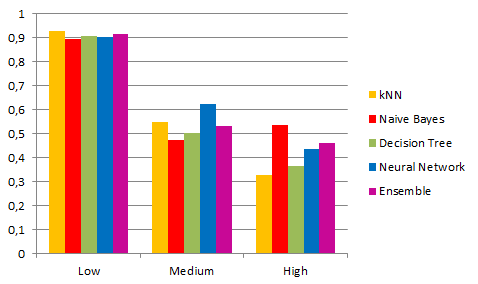
\includegraphics[width=\columnwidth]{../../charts/recall.png}
	\caption{Recall of the different classifiers}
	\label{fig:recall}
\end{figure}

%% The results of k-Nearest Neighbors are shown in \ref{tab:mat-knn}.

%% \begin{table}[H]
%% 	\centering
%% 	\caption{Confusion matrix of the k-Nearest Neighbors classifier with Manhattan distance}
%% 	\label{tab:mat-knn}
%% 	\resizebox{\columnwidth}{!}{
%% 	\begin{tabular}[c]{c|ccc||c}
%% 		classified \(\rightarrow\) & \textbf{Low} & \textbf{Medium} & \textbf{High} & Total\\ \hline
%% 		Low & \textcolor{blue}{1155} & 101 & 3 & 1259 \\
%% 		Medium & 181 & \textcolor{blue}{304} & 37 & 522 \\
%% 		High & 21 & 112 & \textcolor{blue}{80} & 213 \\ \hline \hline
%% 		Total & 1357 & 517 & 120 & 1994 \\
%% 	\end{tabular}
%% }
%% \end{table}

%% The results of the Na\"ive Bayes classifier are shown in \fref{tab:mat-nb}.
%% \begin{table}[H]
%% 	\centering
%% 	\caption{Confusion matrix of the Na\"ive Bayes classifier}
%% 	\label{tab:mat-nb}
%% 	\resizebox{\columnwidth}{!}{
%% 	\begin{tabular}[c]{c|ccc||c}
%% 		classified \(\rightarrow\) & \textbf{Low} & \textbf{Medium} & \textbf{High} & Total\\ \hline
%% 		Low & \textcolor{blue}{1063} & 183 & 13 & 1259 \\
%% 		Medium & 137 & \textcolor{blue}{282} & 103 & 522 \\
%% 		High & 15 & 68 & \textcolor{blue}{130} & 213 \\ \hline \hline
%% 		Total & 1215 & 533 & 246 & 1994 \\
%% 	\end{tabular}
%% }
%% \end{table}

%% The confusion matrix of the decision tree is illustrated in \fref{tab:mat-tree}.
%% \begin{table}[H]
%% 	\centering
%% 	\caption{Confusion matrix of the decision tree}
%% 	\label{tab:mat-tree}
%% 	\resizebox{\columnwidth}{!}{
%% 	\begin{tabular}[c]{c|ccc||c}
%% 		classified \(\rightarrow\) & \textbf{Low} & \textbf{Medium} & \textbf{High} & Total\\ \hline
%% 		Low & \textcolor{blue}{1135} & 111 & 13 & 1259 \\
%% 		Medium & 194 & \textcolor{blue}{277} & 51 & 522 \\
%% 		High & 23 & 105 & \textcolor{blue}{85} & 213 \\ \hline \hline
%% 		Total & 1352 & 493 & 149 & 1994 \\
%% 	\end{tabular}
%% }
%% \end{table}

%% The results of the neural network classifier can be found in \fref{tab:mat-nn}.
%% \begin{table}[H]
%% 	\centering
%% 	\caption{Confusion matrix of the Neural Network}
%% 	\label{tab:mat-nn}
%% 	\resizebox{\columnwidth}{!}{
%% 		\begin{tabular}[c]{c|ccc||c}
%% 			classified \(\rightarrow\) & \textbf{Low} & \textbf{Medium} & \textbf{High} & Total\\ \hline
%% 			Low & \textcolor{blue}{1128} & 128 & 3 & 1259 \\
%% 			Medium & 168 & \textcolor{blue}{317} & 37 & 522 \\
%% 			High & 12 & 108 & \textcolor{blue}{93} & 213 \\ \hline \hline
%% 			Total & 1308 & 553 & 133 & 1994 \\
%% 		\end{tabular}
%% 	}
%% \end{table}

\subsection{Discussion}

Considering all the evaluation metrics shown in \fref{fig:result}, the Neural Network delivered the best results in every case. Contrary to the initial believe that the majority voting would enhance the results, it turned out that they were merely average. 
 
To compare our results with those of \cite{indian}, it should be considered that on the one hand they used predefined ranges for their classification and on the other hand they used different attributes, mostly focusing on income and education.



